% \setlength{\belowcaptionskip}{0pt} 
% \begin{figure}[htbp]
%     \centering
%     \begin{subfigure}[b]{0.5\textwidth}
%         \centering
%         %\includegraphics[scale = 0.25]{Neurips/Screenshots/gin_drchi_6Classes_30/20_N_P_drichi.png}
%         %
\includegraphics[page=1,width=1.0\textwidth]{Neurips/figures/fig8a}
%         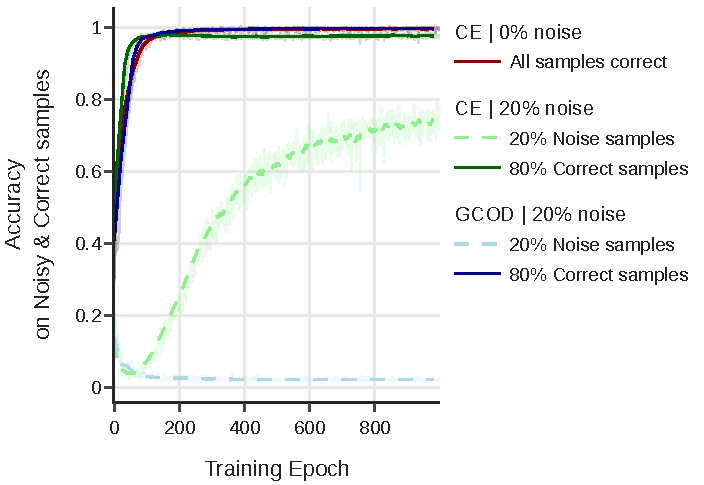
\includegraphics[page=1,width=1.0\textwidth]{AISTATS/figures/fig8a}
%         \caption{Avg. Accuracy for GIN model on the PPA dataset (30\% sample, 6 classes) with clean or 20\% label noise. CE represents Cross Entropy, while \method refers to our modified loss function. 
%         %In particular, we show the average accuracy for three classes ( taken from the 6). For the case with 0\% noise, there are no noisy samples and we reported the accuracy of all samples. For the case of 20\% noise, we reported both the average accuracy of pure samples and the average accuracy of noisy samples.  
%         }
%         \label{fig:PPA_DE_NCOD_subfig1}
%     \end{subfigure}
      
%     \begin{subfigure}[b]{0.5\textwidth}
%         \centering
%         %\includegraphics[scale = 0.25]{Neurips/Screenshots/gin_drchi_6Classes_30/differntnoise_Dirchi_CE_NCOD.png}
%         %
\includegraphics[page=1,width=1.0\textwidth]{Neurips/figures/fig8b}
%         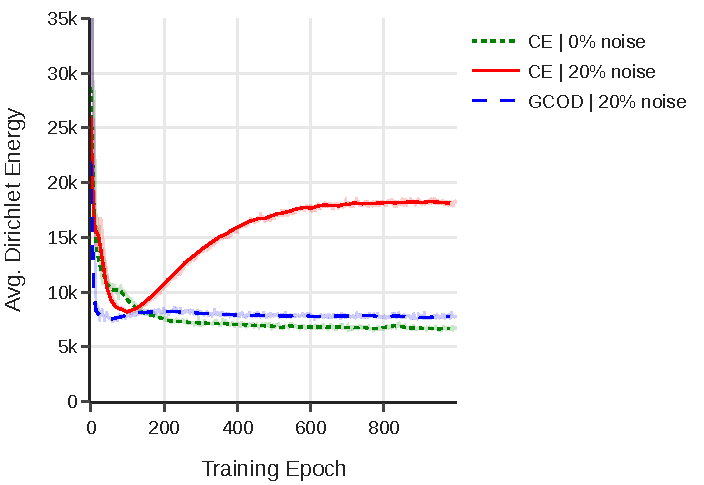
\includegraphics[width=\textwidth]{AISTATS/figures/fig8b}
%         \caption{Evolution of Representation Dirichlet Energy for clean and noise-introduced PPA dataset (30\% sample, 6 classes). Dirichlet Energy increases, when the model with CrossEntropy fits on noise. }
%         \label{fig:PPA_NCOD_Dirich_energy}
%     \end{subfigure}
%     \caption{}
%     % \caption{Illustrates the evolution of both energy and accuracy throughout the training process}
%     \label{fig:mainfig}
% \end{figure}
% Include subfigure package at the beginning of your document


% \begin{figure}[htbp]
%     \centering
%     % \setcounter{figure}{4} 
    
%     \subfigure[Avg. Accuracy for GIN model on the PPA dataset (30\% sample, 6 classes) with clean or 20\% label noise. CE represents Cross Entropy, while \method refers to our modified loss function.]
%     {
%         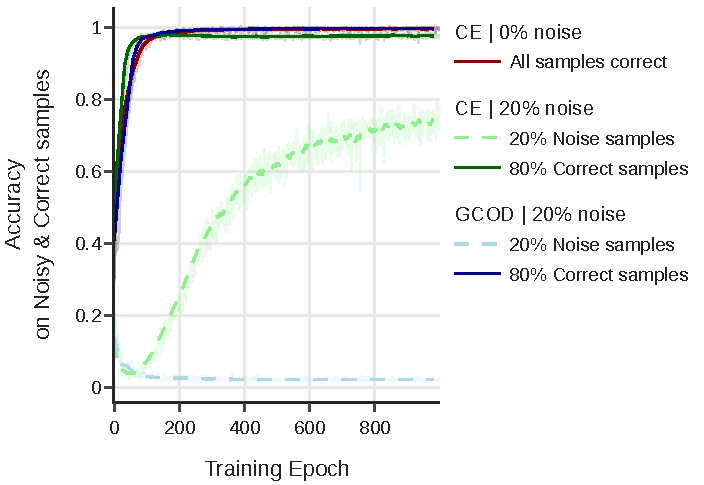
\includegraphics[width=0.45\textwidth]{AISTATS/figures/fig8a}
%         \label{fig:PPA_DE_NCOD_subfig1}
%     }
%     \hfill
%     \subfigure[Evolution of Representation Dirichlet Energy for clean and noise-introduced PPA dataset (30\% sample, 6 classes). Dirichlet Energy increases when the model with CrossEntropy fits on noise.]
%     {
%         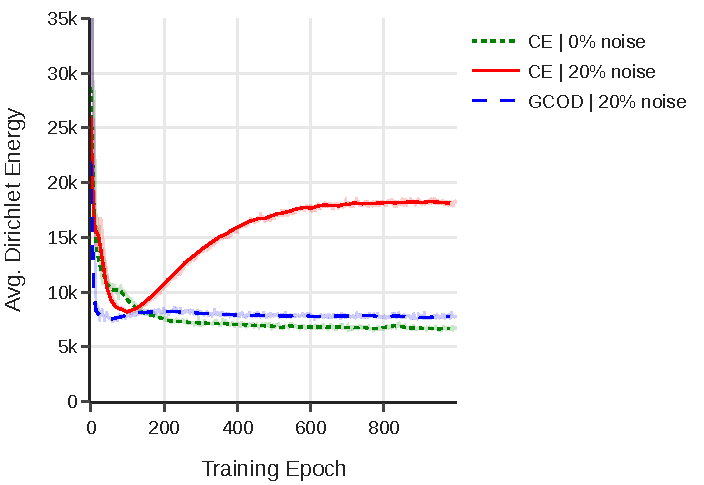
\includegraphics[width=0.45\textwidth]{AISTATS/figures/fig8b}
%         \label{fig:PPA_NCOD_Dirich_energy}
%     }
    
%     % Main figure caption (will still be figure 5)
%     \caption{Illustrates the evolution of both energy and accuracy throughout the training process. Subfigures show: (a) Accuracy trends and (b) Dirichlet Energy evolution.}
%     \label{fig:mainfig}
% \end{figure}


Our previous findings established a strong correlation between a GNN's overfitting of noisy labels and a significant increase in the Dirichlet energy of its learned node representations. 
The spectral properties of the learnable weight matrices within GNN layers fundamentally shape the network's behavior on the graph, particularly concerning smoothing and sharpening of features. Prior work~\citet{noteonoversmoothing, oversmoothing2, GRAFF} has shown that the eigenvalues of learnable weight matrices interact with the graph Laplacian, inducing either smoothing or sharpening effects. In particular, \citet{GRAFF} demonstrates that positive eigenvalues promote attraction between connected nodes, while negative eigenvalues induce repulsion.
These findings suggest that controlling the sign of the weight spectrum could architecturally enforce a smoothing inductive bias. 
This lead us to formulate our second research question: \textbf{RQ2} \textit{Does the spectrum of the weight matrices affect the evolution of \eqref{eq: avg_dirichlet} during training?}



To justify our dataset level analysis of Dirichlet energy, we first present the following result:

\begin{proposition}
\label{theorem: avg_dirichlet}
Let $\mathcal{D} = \{ \mathcal{G}^1= (\mathbf{Z}^1, \mathbf{A}^1), \ldots, \mathcal{G}^{n} = (\mathbf{Z}^n, \mathbf{A}^n) \}$ be a set of graphs. Then
\(
E^{dir}_\text{set}(\mathcal{D}) = \frac{1}{|\mathcal{D}|} E^{dir}(\mathbf{Z}),
\)
where $\mathbf{Z} = [\mathbf{Z^1} \| \ldots \| \mathbf{Z^n}]$ and $\mathbf{A}$ is a block-diagonal matrix with blocks $\mathbf{A}^i$ along the diagonal. That is, the dataset-level Dirichlet energy corresponds to the Dirichlet energy of a single disconnected graph composed of all graphs in $\mathcal{D}$.
\end{proposition} 
\begin{remark}
\label{cor: avg_energy}
Reducing $E^{dir}_\text{set}(\mathcal{D})$ during training implies that the model is simultaneously enhancing low-frequency representations across all graphs in the dataset.
\end{remark}
% \begin{proposition}
% \label{prop: avg_dirichlet}
% Let $\mathcal{D} = \{ \mathcal{G}^1 = (\mathbf{Z}^1, \mathbf{A}^1), \ldots, \mathcal{G}^{n} = (\mathbf{Z}^n, \mathbf{A}^n) \}$ be a collection of graphs. Then the dataset-level Dirichlet energy satisfies
% \[
% E^{\text{dir}}_{\text{set}}(\mathcal{D}) \;=\; \frac{1}{|\mathcal{D}|} \, E^{\text{dir}}(\mathbf{Z}),
% \]
% where $\mathbf{Z} = [\mathbf{Z}^1 \| \cdots \| \mathbf{Z}^n]$ and $\mathbf{A}$ is the block-diagonal adjacency matrix with blocks $\mathbf{A}^i$ on the diagonal.
% \end{proposition}

% \begin{remark}
% \label{rem: avg_energy}
% Minimizing $E^{\text{dir}}_{\text{set}}(\mathcal{D})$ during training enforces smooth, low-frequency representations across all graphs in the dataset simultaneously.
% \end{remark}
Discussion of Proposition~\ref{theorem: avg_dirichlet} and Remark~\ref{cor: avg_energy} is provided in Appendix~\ref{app: proof}.This result supports the idea that smoothing at the dataset level can be induced by controlling the local graph behavior. Motivated by \citet{GRAFF}, we hypothesize that smoothing can be enhanced by removing negative eigenvalues from the learned weight matrices of the GNN. To test this hypothesis, we constrain the spectrum of the weight matrix \( \mathbf{W}^{(2)} \) in each GNN layer after neighborhood aggregation.
% At the end of each training epoch, we:
% \begin{enumerate}
%     \item Compute the eigendecomposition \( \mathbf{W}^{(2)} = \mathbf{Q} \mathbf{\Lambda} \mathbf{Q}^{-1} \),
%     \item Clip all negative eigenvalues: \( \mathbf{\Lambda}_{+} = \max(\mathbf{\Lambda}, 0) \),
%     \item Reconstruct the modified matrix: \( \mathbf{W}^{(2)}_{\text{pos}} = \mathbf{Q} \mathbf{\Lambda}_{+} \mathbf{Q}^{-1} \).
% \end{enumerate}
We refer to this approach as \textbf{CE+W2}, which uses standard cross entropy loss but with post-hoc positive eigenvalue enforcement on \( \mathbf{W}^{(2)} \).
\textit{The full derivation of the update rules, spectrum filtering, and implementation details are provided in Appendix~ \ref{app: weightmatrice_eigens}.} 
The performance of the method is reported in Table~\ref{tab:ppa_30_perc_6_classes}. 
Despite the findings affirm that controlling the weight matrix spectrum influences
Dirichlet energy and robustness, the eigen decomposition step introduces severe training overhead (Table \ref{tab:runtime_comparison}) and potential instability (Appendix Fig. \ref{fig:unstability}).















% In this Section, we propose the following research question: 
% \textbf{RQ2} \textit{Does the spectrum of the weight matrices affect the evolution of \eqref{eq: avg_dirichlet} during training?}

% To answer this and enhance smoothness in the presence of noise, we begin by analyzing the problem from a spectral perspective.
% % To induce smoothness in the presence of noise, we first analyze the problem from a spectral point of view.  
% %As seen in Section \ref{sec:Dirichlet_meet_GC} smoothing adjacent representations corresponds to enhancing the low-frequency components of the node features. 
% %In fact, we can rewrite the Dirichlet Energy in terms of the graph's frequencies eq. \eqref{eq: spectral_dirichlet0}. 
% % Correspondingly, eq.\eqref{eq: avg_dirichlet} may be re-written as:
% % \begin{equation}
% % \label{eq: spectral_avg_dirichlet}
% %    E^{dir}(\mathcal{D}) := \frac{1}{|\mathcal{D}|} \sum_{i = 1}^{n} \sum_{r = 1}^{m} \sum_{u = 1}^{N^i} \lambda_u^i(\bm{\psi}_u^{i,T} \mathbf{Z}^i_{r})^2
% % \end{equation} 
% We show that averaging the Dirichlet Energies of all graphs in the dataset is equivalent to computing the Dirichlet Energy on a single large graph with all dataset samples included as disconnected components, fractioned by ${|\mathcal{D}|}$. Essentially, the set of $n$ graphs can be viewed as one graph with $n$ disconnected subgraphs, each processed separately.
% The proof of the Theorem is in Appendix \ref{app: proof}.

% \begin{theorem}
% \label{theorem: avg_dirichlet}
%     $E^{dir}_\text{set}(\mathcal{D})$ computed on a set of graphs $\{\mathcal{G}^1= (\mathbf{Z}^1, \mathbf{A}^1), \ldots, \mathcal{G}^{n} = (\mathbf{Z}^n, \mathbf{A}^n)\}$ corresponds to  $\frac{1}{|\mathcal{D}|} \cdot E^{dir}(\mathbf{Z})$ of a graph $\mathcal{G} = (\mathbf{Z}, \mathbf{A})$, where $\mathbf{Z} = [\mathbf{Z^1} \|\ldots \| \mathbf{Z^n}]$, and $\mathbf{A}$ is a diagonal block matrix, with diagonal blocks $\mathbf{A}^i, i \in [ n] $.
% \end{theorem}

% \begin{corollary}
% \label{cor: avg_energy}
%     Reducing $E^{dir}_\text{set}(\mathcal{D})$ as the training epochs advance implies that the model learns to enhance simultaneously the low-frequency components of the node features for all graphs in the dataset.
% \end{corollary}
% % We already made an observations that decreasing $E^{dir}(\mathcal{D})$ improves smoothness of all the graphs in $\mathcal{D}$ (see the previous section).
% % Now 


% %According to Corollary \ref{cor: avg_energy}, we can also claim that decreasing $E^{dir}(\mathcal{D})$ corresponds to enhancing the low-frequency components of a single graph which is composed of all disconnected samples in $\mathcal{D}$. 



% Recently, it was shown that interactions between the Laplacian's eigenvalues and eigen spectra of the learnable weight matrices may be responsible for the node features evolution, and thus the Dirichlet Energy evolves as well \cite{noteonoversmoothing, oversmoothing2, GRAFF}. 
% In \cite{GRAFF}, the authors show that in graph convolutions  the symmetric weight matrices can induce attraction (repulsion) on the edges via their positive (negative) eigenvalues. 
% %Specifically, they show that the edge-gradient shrinks along the eigenvectors of the weight matrix associated with positive eigenvalues - i.e., connected nodes' features become more similar, and the Dirichlet Energy tends to decrease. 
% %Conversely, the edge gradient expands along the eigenvectors associated with negative eigenvalues of the weight matrix - i.e., connected nodes' features diverge, and the Dirichlet Energy increases.
% \cite{GRAFF} show that the eigenvalues of the weight matrices determine smoothing or sharpening effects on the node features. Given our Theorem \ref{theorem: avg_dirichlet} we can extend these findings to entire datasets, considering each as a single large graph.

% %Namely, we studied if it was possible to induce smoothing behavior in Eq.~\eqref{eq: avg_dirichlet}, regardless of the presence of noise in the training samples, by directly manipulating the spectrum of the weight matrices by removing negative eigenvalues and reconstructing the weight matrix only with eigenvectors related to positive eigenvalues.
% Specifically, we investigate how to maintain the smoothing bias in Eq.~\eqref{eq: avg_dirichlet} by directly manipulating the spectrum of the GNN weight matrices. This should be independent from presence of noise in a dataset or its properties. For this, we remove the GNN weight matrix negative eigenvalues and reconstructing this weight matrix only with eigenvectors related to its positive eigenvalue.
% Success of this method implies that through our architectural bias, we promote feature smoothing and mitigate the impact of noisy samples. Crucially, this does not require a noise-handling mechanisms. To the best of our knowledge, we are the first to address noise robustness in graph classification tasks by operating at the level of weight matrices from a spectral perspective.

% To address \textbf{RQ2}, we conducted multiple experiments using modified GNN architectures (details in Appendix \ref{app: weightmatrice_eigens}). The most effective approach was to transform (removing negative eigenvalues and reconstructing the weight matrix with only positive eigenvalues) only the final projection weight matrix (in our case it is \textbf{W2} of each layer), which is applied after neighborhood aggregation (refer to Appendix \ref{app: weightmatrice_eigens} for the layers' update equations). The results for the PPA dataset using the GIN network and \textbf{(CE+W2)} are reported in Table \ref{tab:ppa_30_perc_6_classes}. The complete experimental setup and additional details are in Appendix \ref{app: weightmatrice_eigens}.

% Against this empirical evidence, we can affirmatively answer \textbf{RQ2}. While this method successfully induces the desired smoothness, it is impractical. The time-consuming reconstruction of the weight matrices at each iteration leads to increased training time and convergence instability. 
% Yet, we confirm the on the role of GNN smoothness inductive bias, demonstrate it can be architecturally reinforced, and open route for further improvements.
% Thus, remains room for theoretical work.
% to generalize 
% this approach to any message-passing Neural Network.
% which could significantly enhance our understanding of how to bias learning and make GNNs more robust to noise.

 
% \begin{figure}[t!]
%     \centering
%     \begin{subfigure}[b]{0.5\textwidth}
%         \centering
%         %\includegraphics[scale = 0.25]{Neurips/Screenshots/gin_drchi_6Classes_30/20_N_P_drichi.png}
%         %
\includegraphics[page=1,width=1.0\textwidth]{Neurips/figures/fig8a}
%         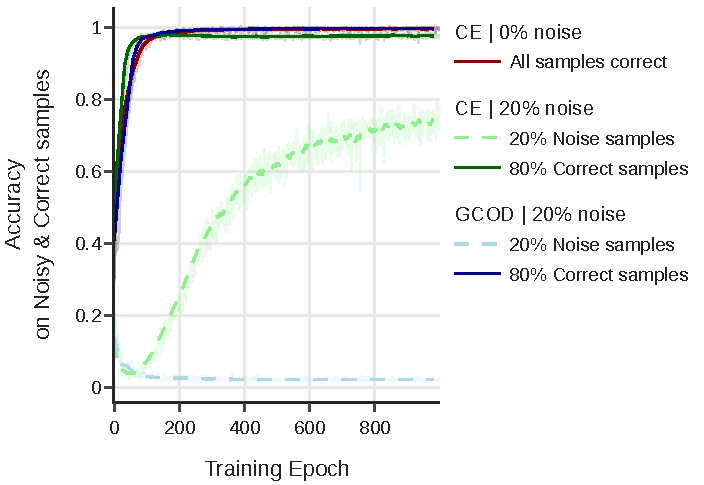
\includegraphics[page=1,width=1.0\textwidth]{AISTATS/figures/fig8a}
%         \caption{Avg. Accuracy for GIN model on the PPA dataset (30\% sample, 6 classes) with clean or 20\% label noise. CE represents Cross Entropy, while \method refers to our modified loss function. 
%         %In particular, we show the average accuracy for three classes ( taken from the 6). For the case with 0\% noise, there are no noisy samples and we reported the accuracy of all samples. For the case of 20\% noise, we reported both the average accuracy of pure samples and the average accuracy of noisy samples.  
%         }
%         \label{fig:PPA_DE_NCOD_subfig1}
%     \end{subfigure}
%        \vspace{0.5cm}


%     \begin{subfigure}[b]{0.5\textwidth}
%  \centering
%         %\includegraphics[scale = 0.25]{Neurips/Screenshots/gin_drchi_6Classes_30/differntnoise_Dirchi_CE_NCOD.png}
%         %
\includegraphics[page=1,width=1.0\textwidth]{Neurips/figures/fig8b}
%         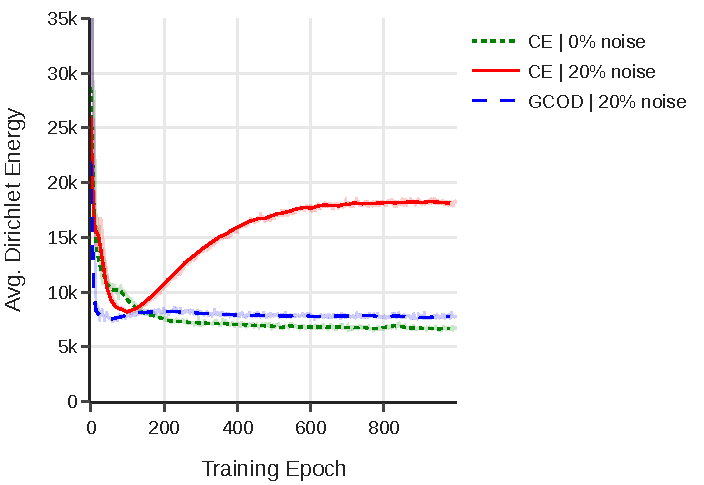
\includegraphics[width=\textwidth]{AISTATS/figures/fig8b}
%         \caption{Evolution of Representation Dirichlet Energy for clean and noise-introduced PPA dataset (30\% sample, 6 classes). Dirichlet Energy increases, when the model with CrossEntropy fits on noise. }
%         \label{fig:PPA_NCOD_Dirich_energy}
%     \end{subfigure}
%     \caption{Illustrates the evolution of both energy and accuracy throughout the training process}
%     \label{fig:mainfig}
% \end{figure}


% \textbf{Experimental setting. }To answer \textbf{RQ2} we conduct the following experiment.
% Let us take the GCN \cite{gcn} update rule for each graph $i$ according to our notation, and write it as: 
% \begin{equation}
%     \text{GCN: \hspace{0.5cm}}
%     \mathbf{H}_i^{l+1} = \sigma(\mathbf{\Delta}\mathbf{H}_i^{l}\mathbf{W}^1_l)\mathbf{W}^2_l \text{\hspace{1cm}} \forall i = \{1, \ldots, n\},
% \end{equation}
% where $\sigma$ is a point-wise non-linearity, and $\mathbf{W}_l^v \in \mathbb{R}^{m' \times m'}$, $v \in \{1, 2\}$ are squared matrices. Moreover, we include $\mathbf{W}_l^2$ for the purpose of the experiments, we can think of it as an additional shallow layer after the message-passing update. Then we consider the GIN \cite{WL1} update rule as: 
% \begin{align*}
%     \text{GIN: \hspace{0.5cm}}
%     \mathbf{H}_i^{l+1} = \sigma(\sigma((1 + \epsilon)\mathbf{H}_i^{l} + \mathbf{A}\mathbf{H}_i^{l})\mathbf{W}_{l}^1)\mathbf{W}_{l}^2) \text{\hspace{1cm}} \\
%     \forall i = \{1, \ldots, n\},
% \end{align*}
% also in this case we use the same squared matrices since we want to operate with eigenvalues rather than the singular values. Here we chose $\epsilon$ as a scalar, and a two layers MLP following the aggregation and update steps (i.e. $(1 + \epsilon)\mathbf{H}_i^{l} +\mathbf{A}\mathbf{H}_i^{l}$). 
% Let us now define the set of eigenvalues and eigenvectors respectively for each corresponding weight matrix $v$ as $\{\mu_{0,l}^{v}, \ldots \mu_{m'-1,l}^{v}\}$, $\{\bm{\Phi}_{0,l}^{v}, \ldots \bm{\Phi}_{m'-1,l}^{v}\}$, $v \in \{1, 2\}$. Let us notice that $\mu_{0,l}^v$ can be also negative, conversely from the eigenvalues of $\mathbf{\Delta}$. We conjecture that the interactions that exist among these sets of eigenvalues, with those of the Laplacian may behave similarly to what is observed and proved in \cite{GRAFF}. For instance, they propose using a symmetric weight matrix (i.e. $\mathbf{W} = \mathbf{W}^{\top}$) having the symmetry property leading to a Dirichlet Energy dynamics that can both sharpen or smooth edge gradients, in particular, the sharpening effect is provided by the influence of the negative eigenvalues of the weight matrix. Assuming that this is true regardless of the message-passing and the weights properties, we know that the sharpening effect is related to noisy samples and is not desired within graph classification. Thus we suggest removing manually such negatives.  \\What we do is: First, we decompose each weight matrix in its eigenvectors and eigenvalues components as follows:
% \begin{equation}
%     \mathbf{W}_l^v = \bm{\Phi}_l^v\bm{\mu}_l^v(\bm{\Phi}_l^{v})^{-1}.
% \end{equation}
% Second, we apply a ReLU function $[\cdot]^+$ to $\bm{\mu_l^{v}}$, in order to keep unchanged the positive eigenvalues and bring the negatives to zero. Then the new $\mathbf{W}_l^{v+}$ will be
% \begin{equation}
%     \mathbf{W}_l^{v+} = \bm{\Phi}_l^v[\bm{\mu}_l^v]^+(\bm{\Phi}_l^{v})^{-1}.
% \end{equation}
% In our experiments we repeat this procedure right after having updated the parameters with gradient descent, excluding it from the gradients computed within the back-propagation algorithm.\\


% \textbf{Experimental results. } In our experiments we condition the weight matrices in several ways. Since we do not have a theoretical rule that guides us on which specific weight matrices, identified by $v$ (weight matrix index) and $l$ (layer index) should be conditioned with positive eigenvalues. Accordingly, we decide to apply the conditioning for every value of $v$ and $l$. Specifically, in Table \ref{tab:ppa_30_perc_6_classes}, we present the results achieved for $v = 2$ across all layers $l$ in the GIN network for the PPA dataset.



%and for both GIN and GCN, we distinguish 2 cases, when we modify only the weights with $v = 2$, or also with $v \in \{1, 2\}$. 
% In Table \ref{tab:ppa_30_perc_6_classes}, we have the results achieved with $v = 2$ for the PPA dataset using the GIN network. %Then, in Figure \ref{}, we have the results derived from using $v \in \{1,2\}$. We notice that all these combinations have a significant effect on the control of $E^{dir}(\mathcal{D})$.

% Consequently, we can positively answer \textbf{RQ2} based on our empirical evidence.
% \textcolor{red}{Use this space to say this strategy is not stable, in what is not stable etv. then uyou can say there is a space for imporvement...  }

%However, a closed-form equation that properly describes the interactions between the two spectra is missing. There is still room for theoretical work to generalize this approach to any message-passing rule. We believe that this direction would have a significant impact on understanding how we can bias our learning and make GNNs more robust to noise.

% As expected the eigenvalues of the weight matrices interact with the Laplacian eigenvalues, which we know are only responsible for smoothing the features. Our general understanding of the results is that indeed, we see that by using only the positive eigenvalues of the weight matrix, the model emphasizes smoothing and discourages fitting noise. Here we conclude that positive eigenvalues promote the diffusion of information across neighboring nodes, leading to smoother feature representations. Consequently, the model focuses on capturing the underlying structure of the graph, leading to a decrease in the Dirichlet Energy and discarding the bad influence of noisy samples. Therefore we can positively answer to \textbf{RQ2} through our empirical evidence. However, a closed form equation that describes properly the interactions between the two spectra is missing, or in general, there's still space for theoretical works that generalize this approach to any message-passing rule. We firmly believe that this direction would have a significant impact on understanding how we can bias our learning and make GNNs more robust to the uncertainties of real-world scenarios.

% Incorrectly labeled nodes introduce discrepancies in the feature space, leading to an increase in 
% \[
% \| F_i - F_j \|^2
% \]
% for nodes that should have similar features.

% \subsection*{Energy Increase}

% As the model tries to fit these incorrect labels, the Dirichlet Energy increases:
% \[
% E_{\text{Dir}}(F) = \sum_{i, j} A_{ij} \| F_i - F_j \|^2 \rightarrow \text{increase}
% \]

% \subsection*{Overfitting to Noise}

% The model overfits to the noise, increasing the high-frequency components of the graph signal, resulting in higher Dirichlet Energy.


% To prevent the model from fitting noise, we consider using only the positive eigenvalues of the weight matrix \(W\).
% Decompose 
% \[
% W = \Theta_+^T \Theta_+ - \Theta_-^T \Theta_-
% \]
% where \(\Theta_+\) and \(\Theta_-\) capture positive and negative eigenvalues, respectively.

% \subsection*{Effect of Positive Eigenvalues}

% Using only the positive part, 
% \[
% W_+ = \Theta_+^T \Theta_+
% \]
% leads to:
% \[
% E_{\text{Dir}}(F') = \text{Tr} \left( (A F W_+)^T \Delta (A F W_+) \right) = \text{Tr} \left( F^T A^T W_+^T \Delta W_+ A F \right)
% \]

% \subsection*{Minimization of Dirichlet Energy}

% Since \(W_+\) has only positive eigenvalues, it promotes smoothing, minimizing 
% \[
% \text{Tr}(F^T \Delta F):
% \]
% \[
% E_{\text{Dir}}(F') \approx \sum_i \left( 1 + \tau \mu_i (1 - \lambda_i) \right)^2 \| F_i \|^2
% \]

% \subsection*{Avoiding Overfitting}

% By eliminating the negative eigenvalues, the model focuses on smoothing and avoids fitting high-frequency noise, thus decreasing \(E_{\text{Dir}}\).

% Prove that smoothness makes sense in the 

% %\section{Main }


% This is a sketch of what we want to say: 



% Graph Neural Networks (GNNs) do not achieve 100\% accuracy, as evidenced by performance on datasets such as the Protein-Protein Association (PPA) dataset. 


% What we noticed in practice is that when noise is introduced to these datasets where the model is not reaching high accuracy, the model that was already struggling to fit clean data will not fit noisy data.